\chapter*{Week 5: Loops}
\addcontentsline{toc}{chapter}{Week 5: Loops}
\setcounter{chapter}{5}
\setcounter{section}{0}

\begin{abstract}
This week you will:
\begin{enumerate}
    \item Learn about while loops
    \item Learn about do-while loops
    \item Learn about for loops

\end{enumerate}
    
\end{abstract}

\section{Background}
Loops are a tool that allows us to repeat a block of code. The number of repetitions is controlled by the conditions of the loop, and can range anywhere from never executing, executing a fixed number of times, or executing an infinite number of times. Loops will execute for as long as their condition is satisfied; once the condition is not true, the loop will stop and the program will continue. The structure of these conditions can vary depending on the type of loop used. There are three main types of loop we use in C++; the while loop, the do-while loop, and the for loop.

\subsection{While Loops}
While loops are the most basic form of loops. Their structure looks like:

\begin{minted}{c++}
while (condition)
{
    //code to execute
}
\end{minted}

Here, $while$ is a C++ reserved word, $condition$ should be a Boolean expression that will evaluate to either \textbf{true} or \textbf{false}, and the comment between the brackets is where we would add code to execute. If the condition is true, then the specified statement(s) within the loop are executed. After running once, the Boolean expression is re-evaluated. If the condition is true, the specified statement(s) are executed again. This process of evaluation and execution is repeated until the condition becomes \textbf{false}.

\begin{example}
Here is an example of a while loop where the condition is based on user input. 
\begin{minted}{c++}
int userChoice = 1;
while (userChoice != 0)
{
   cout << "Do you want to see the question again?" << endl; 
   cout << "Press 0 if no, any other number if yes." << endl;
   cin >> userChoice;
}
\end{minted}
Entering 0 will terminate the loop, but any other number will cause the loop to execute again. Note how we must initialize the condition before the loop starts. Setting userChoice = 1 ensures that the while loop will run at least once.
\end{example}

\begin{example}
    Here is an example of a while loop where the condition is based on a counter.
    \begin{minted}{c++}
int i = 0; 
while (i < 5)
{
    cout << i << endl;
    i = i + 2;
}
    \end{minted}
    Notice how you must manually initialize i=0 and then manually increment i by 2.
\end{example}

\subsection{Do-While Loops}
The do-while loop is a variant of the while loop. The critical difference with a do-while loop is that the block of code we wish to execute is written before the condition. The structure of a do-while loop looks like this:
\begin{minted}{c++}
do {
  // code block to be executed
}
while (condition);
\end{minted}

In a do-while loop, the block of code is executed once before the condition is checked. This means we will never entirely skip a do-while loop. You will often find this type of loop to be useful when gathering user input, like the example shown below.

\begin{example}
    Here is an example of the while loop from example 1.1.1. rewritten as a do-while loop.

    \begin{minted}{c++}
int userChoice;
do {
   cout << "Do you want to see the question again?" << endl; 
   cout << "Press 0 if no, any other number if yes." << endl;
   cin >> userChoice;
}  
while (userChoice != 0);
    \end{minted}

    Note that here we do not have to initialize user choice before the loop begins.
    
\end{example}


\subsection{For Loops}
You will frequently come across instances where you already know the number of iterations you would like your loop to complete, like example 1.1.2 shown above. In these cases, there is a special loop that has a counter built in rather than needing to keep track on your own. For loops have three elements:
\begin{itemize}
    \item Initialization: It must initialize a counter variable to a starting value. Note: When initializing your counter, you can choose to either declare a new variable or use an existing variable. If you declare a new variable in your initialization, it will only exist in the \textbf{scope} of the loop; this means once the loop concludes, you cannot access that variable again. 
    \item Condition: If it is true, then the body of the loop is executed. If it is false, the body of the loop does not execute and jumps to the next statement(s) just after the loop.
    \item Update: Updates the counter variable during each iteration
\end{itemize}

The basic structure of a for loop looks like this:

\begin{minted}{c++}
for (initialization; condition; update)
{
    //code to execute
}
\end{minted}

Here, $for$ is a C++ reserved word. 

\begin{example}
    Here is a section of code that will simply print the word ``hello" five times:
    \begin{minted}{c++}
for (int count = 0; count < 5; count++)
{
    cout << "hello" << endl;
}
    \end{minted}
    Notice the following three parts of the for loop:

    \begin{itemize}
        \item count is initialized to 0,
        \item the conditional expression is count < 5
        \item count++ to increment the count value by one
    \end{itemize}

\end{example}

\begin{example}
    Here is an example that would work equivalently to example 1.1.2.:
    \begin{minted}{c++}
for (int i = 0; i < 5; i = i + 2)
{
    cout << i << endl;
}
    \end{minted}
\end{example}

\subsection{Common Errors and Debugging Loops}

Unique errors with loops include:

\begin{itemize}
\item errors with the loop syntax itself, such as your condition or the set of statements in your for loops. Check that you have semicolons and have declared all your variables that you use in this area. 
\item infinite loops, which will frequently present as either a program that never stops running or an error saying something along the lines of memory exceeded or time exceeded. Check your conditions, and make sure the variables that control your condition are updating correctly. 
\item incorrect numbers of iterations, which means you may not be updating your counter correctly or your logic may be incorrect. 
\end{itemize}
Here is a flowchart for helping you figure out (and resolve) what is wrong with your loops:

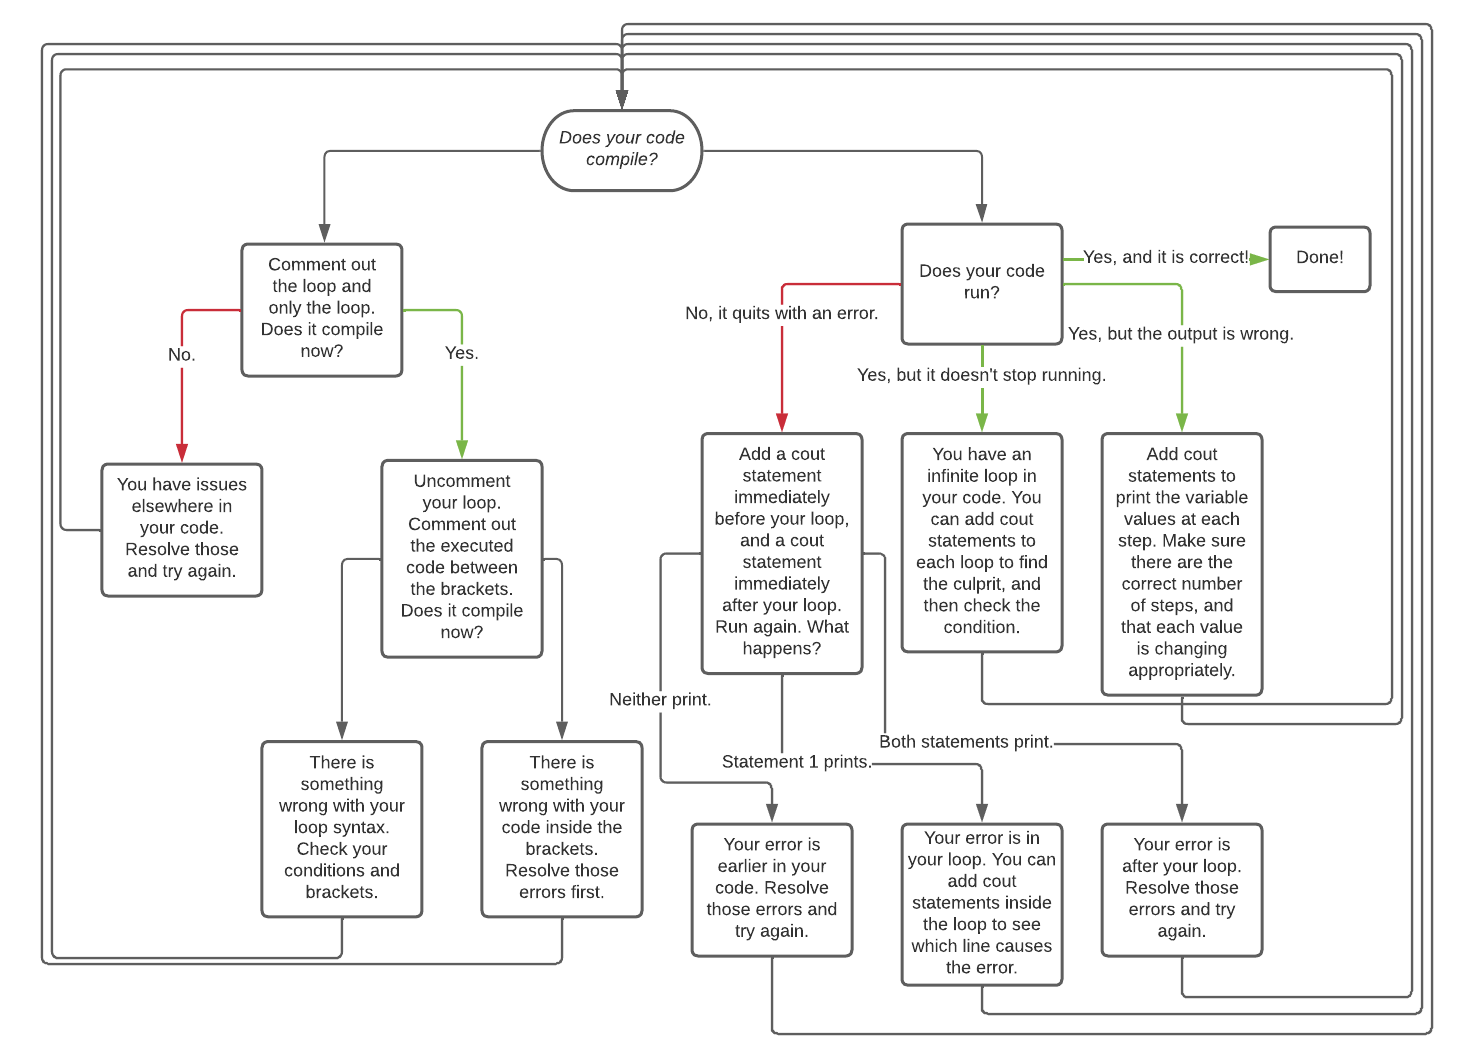
\includegraphics[width=\textwidth]{images/Loop Debugging.png}

Any errors that you may come across either within the bracketed section of your loop or outside of your loop are subject to the same rules as any code we have previously worked with. If you are struggling with errors in those areas, revisit debugging tips from the relevant sections to help you. 

\section{PreQuiz}
\begin{problem} Explain the difference between defining a function and calling a function in C++. Provide an example of each.
\end{problem}

\begin{problem} What does the keyword \texttt{void} signify when used as a function's return type? When would you use it?
\end{problem}

\begin{problem}
In your own words, explain why testing your functions matters. Make sure to mention boundary conditions in your explanation.
\end{problem}

\vspace{5cm}

\begin{problem}
    Fill in the blank(s) for the code below so the function successfully returns the square of the number passed to the function:
    \begin{minted}{c++}
    ______ floatSquare(____ number) {
        return number * number;
    }
\end{minted}

\end{problem}

\begin{problem}
    Fill in the blank(s) for the code below such that the num1 is successfully divided by num2:
    \begin{minted}{c++}
        int integerDivision(______ num1, _____ num2){
            return num1/num2;
        }
    \end{minted}
\end{problem}

\begin{problem}
    Fill in the blank(s) for the code below so that computeArea is successfully called in the blank below, passing in the variables length and width:
    \begin{minted}{c++}
    double computeArea(double length, double width) {
        return length * width;
    }
    
    int main() {
        double length = 5.0;
        double width = 3.0;
    
        // Fill in the blank to call computeArea and store the result
        double area = ______________________________;
    
        cout << "The area is: " << area << endl;
        return 0;
    }
    \end{minted}

\end{problem}

\begin{problem}
Identify the error in the error in our test for the isEven function implemented below:
    \begin{minted}{c++}
    #include <iostream>
    #include <cassert>
    using namespace std;
    
    bool isEven(int num) {
        return num % 2 == 0;
    }
    
    int main() {
        assert(isEven(4) = true);
        return 0;
    }
    \end{minted}
\end{problem}

\section{Recitation}

\subsection{Spot The Error}
\begin{multipart}
The program below will display the average of three values by calling the function \mintinline{c++}{findMean}. Identify the error(s) in the code below, and write the correct line(s).
\end{multipart}

\begin{minted}{c++}
    #include <iostream>
    
    using namespace std;
    
    double findMean(int a, int b, int c)
    {
        int mean = (a+b+c) / 3.0;
        return mean;
    }
    
    int main()
    {
        int average = avg(2,5,2);
        assert(average == 3)
        return 0;
    }
\end{minted}

\begin{multipart}
The program below checks if the two strings given are the same. Identify the error(s) in the code below, and write the correct line(s).
\end{multipart}

\begin{minted}{c++}
    #include <iostream>
    #include <string>
    using namespace std;
    
    string passwordMatchCheck(string password, string confirmPassword) 
    {
        return password = confirmPassword;
    }
    
    int main()
    {
       bool passwordMatch = passwordMatchCheck('Good',"Morning");
       cout << passwordMatch << endl;
    }
\end{minted}

\begin{multipart}
 The same company uses a member ID as the username for its employees. The employees all have an eight digit member ID, and the member ID cannot start with a 0.
\end{multipart}

\begin{minted}{c++}
#include <iostream>
#include <cassert>
using namespace std;

bool idLengthCheck(int ID) 
{
    if (ID >= 9999999 || ID < 100000000)
    {
        return true;
    }
    return false;
}

int main()
{
    assert(idLengthCheck(12345678));
    assert(idLengthCheck("123456789") == False);
    return 0;
}
\end{minted}

\begin{multipart}
The program below will use two functions: one to check for password match and another to check if the ID is valid before registering the user. Assume the relevant functions have been defined successfully. Identify the error(s) in the code below, and write the correct line(s).
\end{multipart}

\begin{minted}{c++}
#include <iostream>
#include <string>
#include <cassert>
using namespace std;

bool passwordMatchCheck(char, char);
bool idLengthCheck(char);

int main() {
    int ID;
    string password;
    string confirmPassword;

    cout << "Enter your member ID: ";
    cin >> ID;
    assert(idLengthCheck(ID));
    
    cout << "Enter your password: ";
    cin >> password;

    cout << "Confirm your password: ";
    cin >> confirmPassword;

    if (passwordMatchCheck(password, confirmPassword)) 
    {
        cout << "Password set successfully for " << username << "." << endl;
    } 
    else if (!passwordMatchCheck(password, confirmPassword)) 
    {
        cout << "Passwords do not match." << endl;
    } 
    else if(!idLengthCheck(ID)) 
    {
        cout << "ID is invalid." << endl;
    }

    return 0;
}

bool passwordMatchCheck(string password, string confirmPassword)
{
    // appropriate definitions
}

bool idLengthCheck(string password)
{
    // appropriate definitions
}
\end{minted}



\begin{multipart}
The program below is a working program that uses the \mintinline{c++}{getPrice} function to compute the price of a wall frame of a given area and color. This code does not contain any syntax or logical errors. However, it has multiple style errors making the code very difficult to read. These errors can range from usage of unintended white space to having extraneous variables or clauses in your code. Identify the style error(s) in the code below and rewrite the below code to improve readability.


\end{multipart}

\begin{minted}[breaklines=true]{c++}
#include <iostream>
#include <string>
#include <cassert>
using namespace std;

double getPrice(double area, string color){
assert(area>=0); double cost = 0.0;
if (color == "green"){
    cost = 4; }
    else if (color == "red")
    { cost = 3; } 
    else if (color == "orange")
    {
    cost = 2;
    }
    else if (color == "blue")
    {
        cost = 1;
    } return area * cost;}

int main()
{
    string color, shape;
    int area_choice;
    double radius;
    double area = 0;

cout << "Enter the area of the frame: (1) 5x5 (2) 4x6 (3) 8x10" << endl;
cin >> area_choice;
    assert(
        area_choice == 1 || area_choice == 2 || area_choice == 3
    );
    if(area_choice == 1){area = 5*5; }
    else if (area_choice == 2){area = 4*6; }
    else if (area_choice == 3){area = 8*10; }

cout << "Enter the color of the frame: (green, red, orange, blue): ";
cin >> color;
    assert(
        color == "green" || color == "red" || color == "orange" || color == "blue"
    );

    double price = getPrice(area, color);

    cout << "You will receive a "<< color << " color frame with a price of $" << price << ". ";
    cout << "Thank you for your business."<<endl;

    return 0;
}
\end{minted}

\subsection{Halloween} %maybe rework this to halloween candy?

In the mysterious town of "Mathville", surrounded by eerie forests, the annual "Halloween Night" celebration is approaching. This town is renowned for blending mathematics with the art of candy making, creating unique candies adorned with mathematical designs.

As the spooky mastermind behind this exciting venture, you're tasked with ensuring the success of Halloween Night by calculating the ingredients for your candies. To achieve this, you'll employ two specialized functions to accurately calculate candy volumes of the pumpkin-shaped candies and the witch's hat candies. 

%update wording to be more clear about how the volume and ingredients are related

%specifically instruct students to use the doublesEqual function from the background info for their assert statements

\begin{itemize}
\item Equation for pumpkin candy volume (approximated as an ellipsoid): \textit{Volume} $= \frac{4}{3}\pi a b c$, where $a$, $b$, and $c$ are the radii along the x, y, and z axes respectively.
\item Equation for witch's hat candy volume (approximated as a cone): \textit{Volume} $= \frac{1}{3}\pi r^2 h$, where $r$ is the radius of the base, and $h$ is the height.
\end{itemize}


\begin{minted}[breaklines=true]{c++}
/**
@brief Function to determine the volume of a pumpkin-shaped candy using its radii
@param radiusX Radius along the x-axis
@param radiusY Radius along the y-axis
@param radiusZ Radius along the z-axis
@return double - volume of the pumpkin-shaped candy
*/ double calculateVolumeOfPumpkinCandy(double radiusX, double radiusY, double radiusZ) { // Your code goes here. }

/**
@brief Function to determine the volume of a witch's hat-shaped candy using its base radius and height
@param radius Base radius of the witch's hat-shaped candy
@param height Height of the witch's hat-shaped candy
@return double - volume of the witch's hat-shaped candy
*/ double calculateVolumeOfWitchHatCandy(double radius, double height) { // Your code goes here. }
\end{minted}

\begin{multipart}
    Write out the steps you would use to solve this problem by hand as pseudocode. 
\end{multipart}

\newpage

\begin{multipart}
    Pick two possible inputs for each of your two functions (four total). Follow the steps you wrote for these values to find your result, and verify it.
\end{multipart}

\vspace{8cm}

\begin{multipart}
Translate your inputs and expected outputs into assert statements.
\end{multipart}

\vspace{8cm}

\begin{multipart}
    Translate your pseudocode into a c++ program to solve the above code, using your assert statements in your main function to verify that your program works as expected.
\end{multipart}


\vspace{8cm}


\section{Homework}

\subsection{Secret Code Language}

You have recently been hired to work for a secret organisation where privacy is the topmost priority. The information you have to share with your co-workers is via email but the communication does not happen in regular English. The language you are using shifts each English letter by a fixed number of positions within the alphabet. The shift value can be positive or negative and should wrap around the alphabet if necessary. For example, with a shift of 3, `a’ would be replaced by `g’, `b’ would become `h’, and so on. So in this case, you have to double the shift input you receive and implement it to your alphabet. If the shift is -3, `d’ would be replaced by `x’, `e’ would become `y’, etc. For simplicity, we are only encrypting lowercase letters in this question. This organization uses the \textcolor{cyan}{\href{https://en.wikipedia.org/wiki/Caesar_cipher}{Caesar cipher}} ideology, but doubled. You have to use this function to send message to each other in the organisation. The shift value is supposed to be doubled and added to the original letter of the message. Below is an image of the actual Caesar cipher explained.

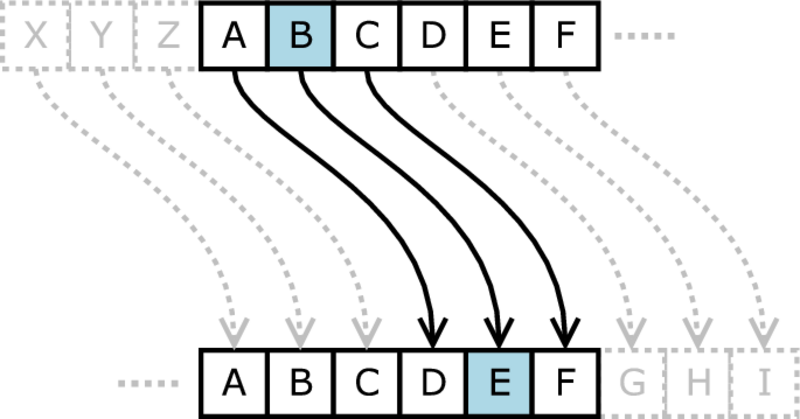
\includegraphics[width=0.8\textwidth]{images/cipher.png}

\bigbreak
\textbf{Note:} Characters like `a' and `z' have specific ASCII values (`a' is 97, `z' is 122). The code uses these values indirectly by operating on character arithmetic rather than directly manipulating ASCII values.
\bigbreak
Write a program that encrypts lowercase letters using the doubled Caesar cipher. Prompt the user for a letter and a shift value in \texttt{main()}, and use the function specification listed below for encryption.


\bigbreak

\begin{longtable}{|p{1.7in}|p{4.0in}|}
\hline
\textbf{Function:} \texttt{encryptLower(char, int)} & \mintinline{c++}{char encryptLower(char letter, int shift_value)}\\ \hline

\textbf{Purpose:} & Encrypt the letter using the shift value. The function should not print anything. \\ \hline

\textbf{Parameters:} & 
\textbf{char} \texttt{letter} - The letter that is being encrypted. \newline
\textbf{int} \texttt{shift\_value} - The shift value that is supposed to be doubled in code. \\ \hline

\textbf{Return value:} & If successful, returns the newly encrypted letter. \\ \hline

\textbf{Error handling/} \newline
\textbf{Boundary conditions:} & 
- If the unencrypted letter is not lowercase, then the unencrypted letter is returned. In other words, return the original letter if it's not lowercase. \newline 
- Hint: You may use the modulo (\%) operation to handle the wrap-around, e.g., if the letter is a and the shift value is -1, the encrypted letter should result in y. \\ \hline

\textbf{Example:} & 
\begin{minted}[breaklines=true]{c++}
// This is only an example usage, and you should develop your own main function
// Assume the proper libraries are included.
// Assume the proper implementation of encryptLower() is included.

int main() {
    char letter = 'r';
    char encrypted_letter = encryptLower(letter, 5);
    cout << "Letter " << letter << " was encrypted to " << encrypted_letter;
    return 0;
}

\end{minted} 

\\ \hline

\textbf{Sample Output (from above example):} & Letter r was encrypted to b \\ \hline

\end{longtable}

Develop and validate your solution in VS Code. Once you are happy with your solution, go to coderunner on Canvas and paste the whole program into the answer box! 


\begin{sample}
Enter the lowercase character to encrypt:

\textcolor{red}{a}

Enter the encryption value:

\textcolor{red}{-1}

Letter a was encrypted to y
\end{sample}

\begin{sample}
Enter the lowercase character to encrypt:

\textcolor{red}{f}

Enter the encryption value:

\textcolor{red}{-3}

Letter f was encrypted to z
\end{sample}

\begin{sample}
Enter the lowercase character to encrypt:

\textcolor{red}{a}

Enter the encryption value:

\textcolor{red}{5}

Letter a was encrypted to z
\end{sample}

\begin{sample}
Enter the lowercase character to encrypt:

\textcolor{red}{a}

Enter the encryption value:

\textcolor{red}{27}

Letter a was encrypted to c
\end{sample}

\begin{sample}
Enter the lowercase character to encrypt:

\textcolor{red}{D}

Enter the encryption value:

\textcolor{red}{10}

Letter D was encrypted to D
\end{sample}



\subsection{Building a Sandcastle}

Imagine you are on a beautiful beach, tasked with building a sandcastle using three different-sized buckets. Each bucket is responsible for creating a specific part of the sandcastle – the castle's towers, walls, and foundation.

At the start, each bucket contains only 1 scoop of sand and fills up at a varying rate. The rate of filling begins at 1 scoop per minute and increases by 2 scoops each minute (for instance, the bucket fills by 1 scoop in the first minute, 3 scoops in the second minute, 5 scoops in the third minute, and so on).

Your objective is to determine how long each bucket needs to be filled to reach the required amounts for the towers, walls, and foundation of the sandcastle. Additionally, calculate the total time required for all three buckets to reach their designated quantities.

\textbf{Note:} Ensure to validate the input size for each part of the sandcastle in \texttt{main()}. If the input is non-positive (i.e., zero or negative), display \texttt{"Please enter a positive integer for <section> size:"}, where <section> refers to the sandcastle part with the incorrect input, and request the user to enter a valid size. This approach guarantees that only valid sizes are accepted for the sandcastle sections.

\begin{longtable}{|p{1.7in}|p{4.3in}|}
\hline
\textbf{Function:}  \texttt{calculateTime(int)} 
& \mintinline{c++}{int calculateTime(int target_size)} \\ \hline

\textbf{Purpose:} & This function calculates the time required for a sandcastle bucket to reach a specified target size. It does not output anything.  \\ \hline

\textbf{Parameters:} & 
\textbf{int} \texttt{target\_size} - The desired size that the sandcastle bucket needs to achieve. \\ \hline

\textbf{Return Value:} & 
Upon successful execution, it returns the time in minutes taken for the sandcastle bucket to reach the desired size. \\ \hline

\textbf{Error Handling:} & The error handling for desired size will occur in \texttt{main()}, which means all target\_size should be valid. \\ \hline

\textbf{Example:} & 
\begin{minted}[breaklines=true]{c++}
// This is a sample usage. You should develop your own main function.
// Assume necessary libraries are included.
// Assume the proper implementation of calculateTime() is provided.

int main() {
    int tower_time = calculateTime(10);
    cout << "Time to reach tower size: " << tower_time << " minutes";
    return 0;
}
\end{minted}
\\ \hline

\textbf{Sample Output (from the example):} & Time to reach tower size: 3 minutes\\ \hline

\end{longtable}

Develop and validate your solution in VS Code. Once you are happy with your solution, go to coderunner on Canvas and paste the whole program into the answer box! 

\begin{sample}

Enter Tower size: \\\textcolor{red}{5}

Enter Wall size: \\\textcolor{red}{7}

Enter Foundation size: \\\textcolor{red}{11}

\\Time to reach Tower size: 3 minutes
\\Time to reach Wall size: 4 minutes
\\Time to reach Foundation size: 6 minutes
\\Total time to create the Sandcastle: 13 minutes

\end{sample}

\begin{sample}

Enter Tower size: \\\textcolor{red}{-12}

Please enter a positive integer for Tower size:

\\\textcolor{red}{15}

Enter Wall size: \\\textcolor{red}{21}

Enter Foundation size: \\\textcolor{red}{27}

\\Time to reach Tower size: 8 seconds
\\Time to reach Wall size: 11 seconds
\\Time to reach Foundation size: 14 seconds
\\Total time to create the Sandcastle: 33 seconds

\end{sample}



\subsection{Print Fibonacci Sequence}

For this question, you will write a program that prompts the user to enter an integer value between 10 and 500 (both exclusive). Your program should then print out a Fibonacci sequence up to the given value following the pattern below:
For a given number $n$,

\begin{itemize}
\item $F_0 = 0, F_1 = 1$
\item $F_n = F_{n-1} + F_{n-2}$ for $n > 1$
\end{itemize}

Your program should stop printing numbers once the sequence reaches a value greater than the given input.

If the user enters a number that is not between 10 and 500 (both exclusive), print ``Invalid input." and prompt the user for a number again.

The Fibonacci sequence is a series of numbers in which each number is the sum of the two preceding ones, usually starting with 0 and 1.

\textbf{Note:} The Fibonacci sequence starts with 0, 1, 1, 2, 3, 5, 8, 13, ...

Develop and validate your solution in VS Code. Once you are happy with your solution, go to coderunner on Canvas and paste the whole program into the answer box!

\begin{sample}
Enter a number between 10 and 500:

\\Invalid input. 
\\Enter a number between 10 and 500: 
\\\textcolor{red}{20} 
0 
1 
1 
2 
3 
5 
8 
13 
Total steps: 8 
\end{sample} 
\begin{sample} Enter a number between 10 and 500: \\\textcolor{red}{122} 
0 
1 
1 
2 
3 
5 
8 
13 
21 
34 
55 
89 
144 
233 
377 
Total steps: 15 
\end{sample}


\subsection{Interest in Baking}
You have a recent interest in Baking cakes where you want to make a few cakes for a party but you have a certain amount of ingredients required and you can bake two types of cakes: Death by chocolate and Black Forest cake. Each type of the cakes require somewhat the same ingredients but in different quantities. The ingredient list looks as follows: Cocoa powder, Vanilla essence, Flour, Whipped cream. 

\bigbreak
Your task is to write a program that asks the user which cake they would like to prioritize the Death by Chocolate cake or Black Forest cake. If the user enters an invalid number for the type of cake, the program should ask them to re-enter like this: ``Invalid input. Please select 1 or 2." The program will prompt the user to input the number of each ingredient they currently have (Cocoa powder, Vanilla essence, Flour, Whipped cream). Based on the available ingredients, calculate how many cakes of the priority type can be made. Any leftover ingredients should be used to make as many of the other type of cake as possible. Finally, the program should output how many of the priority cakes can be crafted and how many of the other cakes can be made with the remaining ingredients. 

The ingredient requirements for each type of cake are as follows:

\begin{table}[H]
    \centering
       \begin{tabular}{|c|c|c|c|}
    \hline
    \textbf{Ingredients} & \textbf{Amount for Death by Chocolate cake } &\textbf{Amount for Black Forest Cake} 
    \\
    \hline
    Cocoa powder & 3 & 1
    \\
    \hline
    Vanilla essence & 2 & 4
    \\
    \hline
    Flour & 6 & 10 \\
     \hline
    Whipped cream & 3 & 2 \\
    \hline
    \end{tabular}

\end{table}

Develop and validate your solution in VS Code. Once you are happy with your solution, go to coderunner on Canvas and paste the whole program into the answer box! 

\begin{sample}
Select your cake making priority:
\\1. Death by Chocolate cake
\\2. Black Forest cake
\\\textcolor{red}{2}
\\How much Cocoa powder do you have?
\\\textcolor{red}{30}
\\How much Vanilla essence do you have?
\\\textcolor{red}{40}
\\How much Flour do you have?
\\\textcolor{red}{12}
\\How much Whipped cream do you have?
\\\textcolor{red}{22}
\\You can make 0 Death by Chocolate cake(s) and 1 Black Forest cake(s).
\end{sample}


\begin{sample}
Select your cake making priority:
\\1. Death by Chocolate cake
\\2. Black Forest cake
\\\textcolor{red}{3}
\\Invalid input. Please select 1 or 2.
\\\textcolor{red}{2}
\\How much Cocoa powder do you have?
\\\textcolor{red}{10}
\\How much Vanilla essence do you have?
\\\textcolor{red}{5}
\\How much Flour do you have?
\\\textcolor{red}{8}
\\How much Whipped cream do you have?
\\\textcolor{red}{3}
\\You can make 1 Death by Chocolate cake(s) and 0 Black Forest cake(s).
\end{sample}

\begin{sample}
Select your cake making priority:
\\1. Death by Chocolate cake
\\2. Black Forest cake
\\\textcolor{red}{1}
\\How much Cocoa powder do you have?
\\\textcolor{red}{10}
\\How much Vanilla essence do you have?
\\\textcolor{red}{15}
\\How much Flour do you have?
\\\textcolor{red}{19}
\\How much Whipped cream do you have?
\\\textcolor{red}{27}
\\You can make 2 Death by Chocolate cake(s) and 0 Black Forest cake(s).
\end{sample}





\subsection{Validate Integer}
Design a function \mintinline{c++}{validateInt} that accepts a string input and determines if it represents a valid integer by checking if each character in the string is a valid value. Your program should ask the user to input an integer, store it as a string, and then invoke the \mintinline{c++}{validateInt} function to check its validity. The program should then print whether the string is a valid integer or not. (Negative integers are also valid integers).


\begin{table}[H]
    \centering
    \begin{tabular}{|p{1.7in}|p{4.3in}|} \hline
        \textbf{Function:} \newline 
        validateInt(string) & \mintinline{c++}{bool validateInt(string input)}\\ \hline
        \textbf{Purpose:}  &  Iterate through a string and verify if it is a valid integer or not. The function should not print anything. \\ \hline
        \textbf{Parameters:} &  \hangindent=1cm \textbf{string} \texttt{input} - The string to be verified  \\ \hline
        \textbf{Return value:} &  It returns true if the string is a valid integer. Otherwise, it returns false. \\ \hline
        \textbf{Error handling/} \newline
        \textbf{Boundary conditions:} & If length of input = 0, false is returned  \\ \hline
        \textbf{Example:} & 
        \begin{example}
            \begin{minted}[breaklines=true]{c++}
            
// Assume the proper libraries are included.

// Assume the proper implementation of validateInt() is included.

int main()
{
    string number;
    cout << "Enter the integer : " << endl;
    getline(cin, number);
    if(!validateInt(number))
    {
        cout << "The entered string is not a valid integer!!" << endl;
    }
    else
    {
        cout << "The entered string is a valid integer!!" << endl;
    }
    return 0;
}
            \end{minted}
        \end{example}

        \begin{sample}
Enter the integer :

\textcolor{red}{1234}

The entered string is a valid integer!!
        \end{sample}
             \\ \hline
    \end{tabular}
\end{table}

Develop and validate your solution in VS Code. Once you are happy with your solution, go to coderunner on Canvas and paste just the \texttt{validateInt()} function into the answer box! 

\begin{sample}
Enter the integer :

\textcolor{red}{-12}

The entered string is a valid integer!!
\end{sample}

\begin{sample}
Enter the integer :

\textcolor{red}{23e56}

The entered string is not a valid integer!!
\end{sample}

\begin{sample}
Enter the integer :

\textcolor{red}{32 56}

The entered string is not a valid integer!!
\end{sample}

\begin{sample}
Enter the integer :

\textcolor{red}{-}

The entered string is not a valid integer!!
\end{sample}

\begin{sample}
Enter the integer :

\textcolor{red}{456789}

The entered string is a valid integer!!
\end{sample}